\section{EP-Launch Program}\label{ep-launch-program}

EP-Launch is an optional component of the EnergyPlus Windows installation (it is not available for Linux and Mac platforms). For users that want a simple way of selecting files and running EnergyPlus, EP-Launch provides this and more. In addition, EP-Launch can help open a text editor for the input and output files, open a spreadsheet for the postprocessor results files, a web browser for the tabular results file, and start up a viewer for the selected drawing file.

\begin{figure}[hbtp] % fig 4
\centering
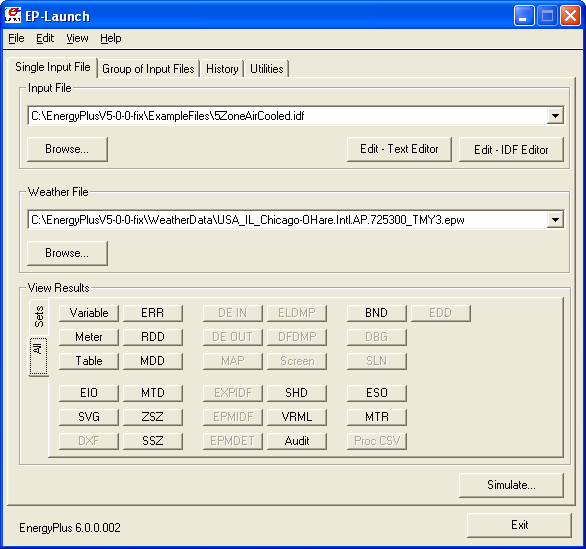
\includegraphics[width=0.9\textwidth, height=0.9\textheight, keepaspectratio=true]{media/image004.png}
\caption{EP-Launch Screen \protect \label{fig:ep-launch-screen}}
\end{figure}

\subsection{Start EP-Launch}\label{start-ep-launch}

EP-Launch is located in the main directory/folder for EnergyPlus. In addition, it is available on the shortcut menu for EnergyPlus.~ By double clicking on the EP-Launch icon you get the screen shown above (Figure~\ref{fig:ep-launch-screen}) for running a single input file. The EP-Launch program simply starts other programs and allows you to avoid having to use the DOS command line prompt to run EnergyPlus. More help is provided for the program under the ``Help'' menu.

\subsection{Selecting Input and Weather Files}\label{selecting-input-and-weather-files}

The input file and weather files can be selected on the Single Input File tab from the two pull down lists which show recently used files or you can press the ``Browse\ldots{}'' buttons to locate an input or weather file that you have created yourself. If this is your first time using EP-Launch, the pull down lists will show some files from the ExampleFiles subdirectory. These are not the only examples, use browse to open other example files from the ExampleFiles subdirectory or other EnergyPlus input files.

\subsection{Running a Single Input File}\label{running-a-single-input-file}

On the Single Input File tab, after you select the weather and input files simply push the ``Simulate\ldots{}'' button to start the EnergyPlus building energy simulation engine. At this point a black DOS window should pop up on your screen and show the progress of your simulation. The simulation is complete when the black DOS box closes. The EnergyPlus program black DOS window will show scrolling text as the simulation procedure progresses. If you would like to see these messages more slowly you have two options:

1)~~~Press the ``Control-S'' key combination to try to stop the progress and any key to continue.

2)~~~Under the ``View'' menu on the EP-Launch program, select ``Options'' then ``Command Window'' then check ``Pause During Simulation'' and this will pause the process immediately after EnergyPlus executes. To continue after the pause, press any key.

If the file contains Parametric objects, the single input file may cause multiple simulations to be performed. If multiple simulations are performed, the output files will be listed on the History tab and will be named with either the file suffixes defined in the input file or with a serial number.

Multiple single input file and group simulations can be started at the same time. On a computer with multiple-processors or multiple-cores, this will enable the simulations to complete more quickly than starting one after another.

\subsection{Looking at the Results}\label{looking-at-the-results}

After you have run a simulation and the black DOS window closes, EnergyPlus has completed, and a status message is displayed see Figure~\ref{fig:ep-launch-finish-status}:

\begin{figure}[hbtp] % fig 5
\centering
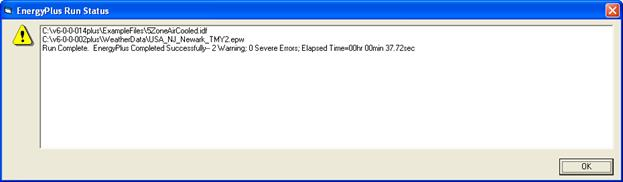
\includegraphics[width=0.9\textwidth, height=0.9\textheight, keepaspectratio=true]{media/image005.jpg}
\caption{EP-Launch Finish Status \protect \label{fig:ep-launch-finish-status}}
\end{figure}

This status gives you a quick overview of whether there were warning (\textbf{should look at}), severe (\textbf{should probably fix}) or fatal (\textbf{must fix}) errors in the run as well as the time it took for the simulation to complete.~ After pressing ``OK'' from this box, selecting ``ERR/EIO/BND Output Files Only'' from the ``View'' menu will display the ERR, EIO, and BND files -- useful when errors may have occurred. Alternatively, pressing the F2 function key will display the same three files.

Another way to open files easily is by using the View Results buttons shown in Figure~\ref{fig:ep-launch-with-the-sets-tab-of-view-results}. Two different panels of buttons can be used under View Results, one shown by using the ``All'' tab on the left edge and by using the ``Sets'' tab on the left edge. The ``All'' tab shows all the various files by file extension that can be viewed individually.~ Files available for view~ based on the current input file name are ``enabled'' (extension names clearly readable). The contents of each file extension is listed below.

\begin{figure}[hbtp] % fig 6
\centering
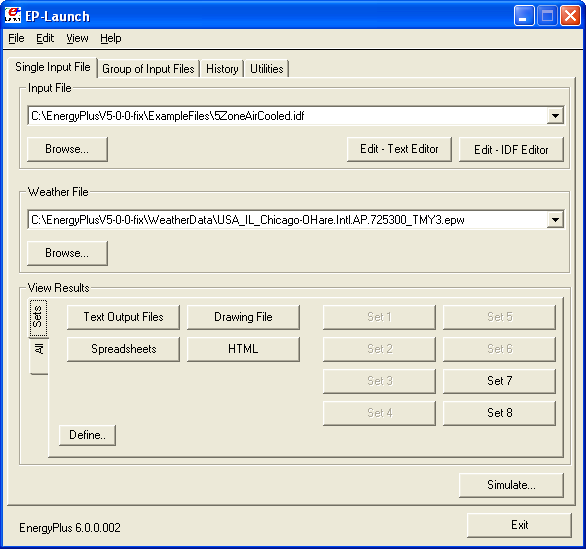
\includegraphics[width=0.9\textwidth, height=0.9\textheight, keepaspectratio=true]{media/image006.png}
\caption{EP-Launch with the Sets tab of View Results \protect \label{fig:ep-launch-with-the-sets-tab-of-view-results}}
\end{figure}

The figure above shows the same main screen of EP-Launch but with the ``Sets'' tab selected on the left edge of the View Results section. The buttons on this tab can open many files at the same time and are a shortcut to opening the files that may be commonly used. The Text Output Files, Drawing Files, and Spreadsheets buttons cause several different results files to open at once based on the currently selected Input File. The HTML file opens just the tabular results file if that file was produced (see \emph{OutputContol:Table:Style}).

The contents (along with examples) are discussed in the \href{file:///E:/Docs4PDFs/OutputDetailsAndExamples.pdf}{Output Details} document.

You can also view the results using one of the three buttons (``Text Output Files,'' ``Drawing File'' and ``Spreadsheets'') in the ``View Results'' area of the main EP-Launch screen.

By pressing the ``Text Output Files'' button, a text editor will open each of the text output files. Up to 29 files will open, if they exist. Selecting ``Single File'' from the `View `` menu displays a menu of all available output files from which any file can be opened individually. Each file may also be opened with an associated function key. The output files and function key shortcuts are listed below:

1.~Variable -- tabulated results in comma, tab or space delimited format (generated by the ReadVarsESO postprocessor) (F4)

2.~ESO -- raw report variable output (F5),

3.~RDD -- list of output variables available from the run (F6).

4.~MDD -- list of output meters available from the run (Shift-Ctrl-F3)

5.~EIO -- additional EnergyPlus results (F7),

6.~ERR -- list of errors and warnings (F8),

7.~BND -- HVAC system node and component connection details (F9),

8.~MTR -- raw report meter output (F11),

9.~MTD -- list of meter component variables (F12)

10.~METER File -- tabulated meter report in comma, tab or space delimited format (generated by the ReadVarsESO postprocessor) (Ctrl-F4)

11.~ZSZ -- zone sizing details in comma, tab or space delimited format (Ctrl+F5)

12.~SSZ -- system sizing details in comma, tab or space delimited format (Ctrl+F6)

13.~AUDIT -- input file echo with input processor errors and warnings (Ctrl+F8)

14.~SLN -- output from ``report, surfaces, lines'' (Ctrl+F9)

15.~DBG -- output from the debug command (Ctrl+F11)

16.~SHD -- output related to shading (Ctrl+F12)

17.~SVG - HVAC Diagram (Shift+ F4)

18.~EPMIDF -- clean idf file after EP-Macro processing (Shift+F5)

19.~EPMDET -- EP-Macro detailed output with errors and warnings (Shift+F6)

20.~MAP -- daylighting illuminance map (Shift+F7)

21.~TABLE -- tabulated report of bin and monthly data in comma, tab or space delimited or HTML format~ (Shift+F8)

22.~VMRL -- drawing file in VRML (Virtual Reality Markup Language) format (Shift F+F11)

23.~DXF -- drawing file in AutoCAD DXF format (Shift+F12)

24.~Delight IN - DElight input generated from EnergyPlus processed input (Shift+Ctrl+F4)

25.~Delight OUT -- Detailed DElight output (Shift+Ctrl+F5)

26.~Delight ELDMP -- DElight reference point illuminance per time step (Shift+Ctrl+F6)

27.~Delight DFDMP -- DElight warning and error messages (Shift+Ctrl+F7)

28.~EXPIDF -- Expanded IDF when using HVACTemplate objects (Shift+Ctrl+F8)

29.~Group Error -- combined error files for a group run. (Shift+Ctrl+F9)

30.~VCpErr -- Transition program error file (Shift+Ctrl+F11)

31.~Screen (Shift+Ctrl+f12)

32.~Proc CSV -- Simple statistiscs generated from CSVProc (also see Create Statistics File option under View-Options).

33.~EDD -- Energy Management System details.

Clicking on the ``Drawing File'' button will open the generated DXF file if an appropriate viewer has been configured (see \emph{Selecting Viewers and Editors} below). The DXF file is a CAD format that displays the physical shape of the building being modeled in three dimensions. The ``Drawing File'' button also opens the HVAC diagram generated with the HVAC-Diagram utility (see Auxiliary Programs).

Clicking on the ``Spreadsheets'' buttons will open any generated CSV files if an appropriate viewer has been configured (see \emph{Selecting Viewers and Editors} below).

\subsection{Viewing the Drawing File without Running a Simulation}\label{viewing-the-drawing-file-without-running-a-simulation}

The ``Drawing'' button (or the View menu Drawing File option) will automatically run EPDrawGUI if the DXF file does not exist or it is older than the input file. This allows the building geometry to be viewed without running a full simulation. For more information about EPDrawGUI, see the \href{file:///E:/Docs4PDFs/AuxiliaryPrograms.pdf}{\emph{Auxiliary Programs}} document.

\subsection{Editing the Input Files}\label{editing-the-input-files}

The input file, called IDF file that is selected from the top pull-down list, can be edited by pressing one of two buttons in the ``Input File'' area. The ``Edit - Text Editor'' button will start a text editor and the ``Edit - IDF Editor'' will start the separate program called the IDF Editor. Remember to save any changes you make in either editor before returning to EP-Launch to run the simulations again.

\subsection{File Menu}\label{file-menu}

The File menu can be used for selecting input and weather files just like the ``Browse\ldots{}'' buttons (see the \emph{Selecting Input and Weather Files} section above).

If you are upgrading from the previous version of EnergyPlus you can use the ``File'', ``Transition'' menu option to upgrade your EnergyPlus input files (IDF and IMF) to the most recent version (see the \href{file:///E:/Docs4PDFs/AuxiliaryPrograms.pdf}{AuxiliaryPrograms} document for more information about the Transition program). This EP-Launch option only works for upgrading input files one version.

\subsection{Edit Menu}\label{edit-menu}

No cutting or pasting is used in this program so the edit menu shows options that duplicate the functions of the ``Edit -- Text Editor'' and ``Edit -- IDF Editor'' buttons. In addition, the weather file and the postprocessor command file (rvi) may be opened in the text editor.

\subsection{View Menu}\label{view-menu}

The View menu (Figure~\ref{fig:ep-launch-view-menu}) duplicates the options in the ``View Results'' area of the main screen (see the \emph{Looking at the Results} section above) and allows opening of selected output files. You can also open the folders that contain the active input and weather files. Opening a single file is under a submenu and is very similar to the Quick Open Panel for Single Simulation described above. Selecting ``HTML File'' from the ``View'' menu will open any user created files saved in the format: \textless{}filename\textgreater{}table.html (see \emph{OutputControl:Table:Style}).

\begin{figure}[hbtp] % fig 7
\centering
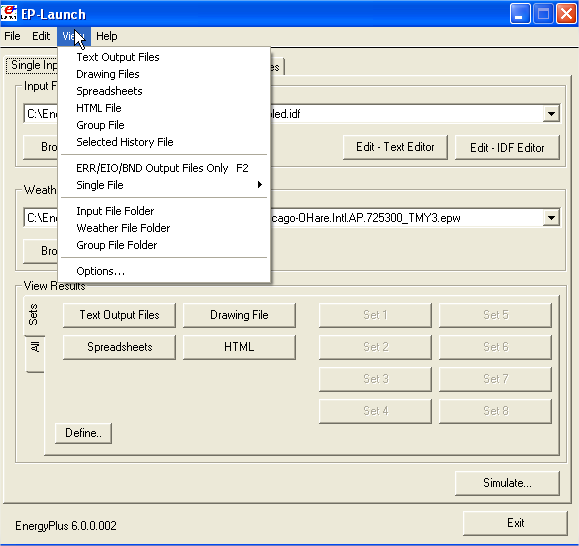
\includegraphics[width=0.9\textwidth, height=0.9\textheight, keepaspectratio=true]{media/image007.png}
\caption{EP-Launch View Menu \protect \label{fig:ep-launch-view-menu}}
\end{figure}

\begin{figure}[hbtp] % fig 8
\centering
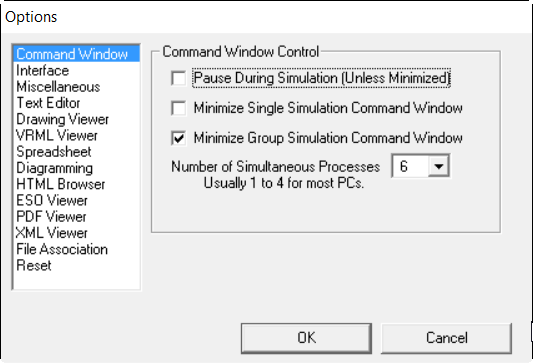
\includegraphics[width=0.9\textwidth, height=0.9\textheight, keepaspectratio=true]{media/image008.png}
\caption{EP-Launch Options Screen. \protect \label{fig:ep-launch-options-screen.}}
\end{figure}

The ``View'' menu also accesses the ``Options'' menu item shown in Figure~\ref{fig:ep-launch-options-screen.} that is used to control many of the optional features of EP-Launch. These optional features are described below:

\subsubsection{Command Window Options}\label{command-window-options}

\textbf{Pause During Simulation (Unless Minimized)} -- Stops the progress of the EnergyPlus run at different points. This does not stop the simulation itself but pauses before or after important events as files are copied or utility programs are run. It is usually used only for diagnosing problems with the EPL-RUN batch file. The feature is also described in the \emph{Running a Single Input File} section above.

\textbf{Minimize Single Simulation Command Window} -- For a single input file, minimizes the Command Window that EP-Launch uses to run EnergyPlus. The command window will appear only in the Windows taskbar and the command window will not be visible. You can restore the command window be clicking on the taskbar item labeled ``EnergyPlus Process''. This option should be used with caution since you will not see any indication of the simulation being complete other than the ``EnergyPlus Process'' taskbar item will disappear.

\textbf{Minimize Group Simulation Command Window} -- For a group of input files, minimizes the Command Window that EP-Launch uses to run EnergyPlus. This is a good option when working on something else on your computer at the same time as the group of simulations is running since the command window normally becomes the front window each time a new simulation starts. This option prevents the command window coming to the front for each simulation. The command window will appear only in the Windows taskbar and the command window will not be visible. You can restore the command window be clicking on the taskbar item labeled ``EnergyPlus Process''. This option should be used with caution since you will not see any indication of the simulation being complete other than the ``EnergyPlus Process'' taskbar item will not be present.

\textbf{Number of Simultaneous Processes} -- Select the maximum number of simulations that should be able to be run at the same time. For a computer with multiple processors or multiple cores, this will allow better utilization of the computers power. The value selected should correspond to the number of processors/cores but higher or lower number can be used as well.

\subsubsection{Interface Options}\label{interface-options}

\textbf{Extra Wide Window} -- Select this option to make the main EP-Launch window wider. This is useful when files are used with very long file path names.

\textbf{Alternative layout} -- Changes the layout of the EP-Launch window to an alternative arrangement of buttons.

\subsubsection{Miscellaneous Options}\label{miscellaneous-options}

\textbf{Tab Delimited Open with Spreadsheet} -- Selecting ''Single File'' and then ``Main Results File'' from the ``View'' menu or pressing the F4 function key will open TAB files with the default spreadsheet application rather than the text editor. Comma-separated variable (CSV) is the default setting for viewing tabulated results set in the RVI file. If the user changes the setting for viewing tabulated results to TAB or TXT format, selecting ''Single File'' and then ``Main Results File'' from the ``View'' menu or pressing the F4 function key will open the files in the default text editor.~ TAB files, when selected, will also be opened by the text editor when the ``Text Output Files'' button is pressed after a successful run.

\textbf{Allow More Than 250 Columns} -- Tabulated data that exceeds 250 columns, the MS Excel maximum, will be truncated to that limit unless ``Allow \textgreater{}250 Columns'' is selected. Excel versions prior to 2007 were limited to 255 columns in a sheet; later versions allow unlimited number of columns. This limitation may not be true for other spreadsheet programs.

\textbf{Check VERSION Prior to Simulation} -- Automatically check the VERSION object in the selected EnergyPlus input file prior to simulation and if it is an older version than the current version will run the Transition program to update the file.

\textbf{Convert ESO/MTR to IP Units} -- Runs the convertESOMTR utility program (see AuxiliaryPrograms documentation for more information). This utility will convert the ESO and MTR files into Inch-Pound units. The CSV file created from these files will also be in Inch-Pound units.

\textbf{Create Statistics File} -- Runs the CSVProc utility program (see the AuxiliaryPrograms documentation for more information) and creates the --Proc.csv file. This file contains some simple statistics on each variable in the normal CSV file.

\textbf{Create Batch File to Run EnergyPlus} -- Traditionally EP-Launch has created a batch file in order to execute EnergyPlus with the various options chosen. This can cause problems with some operating systems, such as Windows Vista, when set to a higher security setting.~ This option can be unchecked and a batch file is not created when running EnergyPlus instead parameters are passed to an existing batch file.

\textbf{Run ParametricPreprocessor} -- When this option is checked, if Parametric objects are present in the file, the ParametricPreprocessor will be run prior to the first simulation and if multiple simulations are needed they will all be executed. See the Auxiliary Programs documentation for details.

\textbf{Check for Updates to EnergyPlus} -- When this option is checked, EP-Launch will check every seven days if an update to EnergyPlus or any of the files distributed with EnergyPlus are available to download. If they are available a message will be shown upon start up.~ You can also manually check by going to HELP .. CHECK FOR UPDATES.

\subsubsection{Text Editor Options}\label{text-editor-options}

EP-Launch will start a text editor when editing a IDF file or when viewing many of the results files.~ The text editor that will be used is shown but can be changed by either pressing the Select button or by pressing the Auto Find button. The Select button allows you to find the text editor of your choice. The Auto Find button will automatically find the program that is associated with the TXT file extension and use that program. Auto Find is invoked the first time EP-Launch is started so that a text editor is available immediately. The most common text editor is NOTEPAD.EXE and is built into Windows but many other text editors are also available.

\subsubsection{Drawing Viewer Options}\label{drawing-viewer-options}

The default drawing viewer is the application associated with DXF files. This can be changed to your favorite drawing program by using the Select button then locating the executable file for your favorite drawing software capable of reading a DXF file. The Auto Find button will automatically find the program that is associated with the DXF file extension and use that program. A variety of programs (free of charge) can render DXF files for viewing.~ The \href{file:///E:/Docs4PDFs/OutputDetailsAndExamples.pdf}{Output Details} document lists some of these programs as well as displaying what a DXF rendered file looks like on the screen.

\subsubsection{VRML Viewer Options}\label{vrml-viewer-options}

EP-Launch will start a VRML Viewer when a building drawing is created using the Report, Surfaces, VRML option in your IDF file.~ The VRML Viewer that will be used is shown but can be changed by either pressing the Select button or by pressing the Auto Find button. The Select button allows you to find the VRML Viewer of your choice. The Auto Find button will automatically find the program that is associated with the WRL file extension and use that program. Auto Find is invoked the first time EP-Launch is started so that a VRML Viewer is available immediately. Many other VRML Viewers are available.

\subsubsection{Spreadsheet Options}\label{spreadsheet-options}

EP-Launch will start a spreadsheet program when viewing many of the results files.~ The spreadsheet that will be used is shown but can be changed by either pressing the Select button or by pressing the Auto Find button. The Select button allows you to find the spreadsheet program of your choice. The Auto Find button will automatically find the program that is associated with the CSV file extension and use that program. Auto Find is invoked the first time EP-Launch is started so that a spreadsheet program is available immediately.

\subsubsection{Diagramming Options}\label{diagramming-options}

EP-Launch will start a diagramming program to view SVG files from HVAC Diagram.~ The diagramming program that will be used is shown but can be changed by either pressing the Select button, the Auto Find button, the Use Firefox button or the Use Opera button. The Select button allows you to find the diagramming program of your choice but make sure it is capable of opening SVG files. The Auto Find button will automatically find the program that is associated with the SVG file extension and use that program. Auto Find is invoked the first time EP-Launch is started so that a spreadsheet program is available immediately.~ Since both Firefox and Opera web browsers can view SVG files, those buttons will select those respective browsers if available.

\subsubsection{HTML Browser Options}\label{html-browser-options}

EP-Launch will start a HTML browser program when viewing the tabular results file when HTML is chosen in OutputControl:Table:Style object. The HTML browser that will be used is shown but can be changed by either pressing the Select button or by pressing the Auto Find button. The Select button allows you to find the HTML browser of your choice. The Auto Find button will automatically find the program that is associated with the HTML file extension and use that program. Auto Find is invoked the first time EP-Launch is started so that a HTML browser is available immediately.

\subsubsection{ESO Viewer Options}\label{eso-viewer-options}

By default, ESO files are opened with a text editor. ESO files are the raw output file containing results from EnergyPlus for Output:Variable objects. They are often processed into CSV files to make it easier to view them. At least one utility program has been developed to view ESO files directly (see the EnergyPlus.gov web site under ``Interfaces \& Other Tools'', ``Third-party EnergyPlus Tools).~ The Auto Find and Select buttons work the same way as other viewer selectors. If no special ESO viewer is selected the box will be shown as empty. It can also be emptied by using the Clear button.

\subsubsection{PDF Viewer Options}\label{pdf-viewer-options}

EP-Launch will start a PDF viewer program when opening the EnergyPlus documentation under the Help menu.~ The PDF Viewer that will be used is shown but can be changed by either pressing the Select button or by pressing the Auto Find button. The Select button allows you to find the PDF Viewer of your choice. The Auto Find button will automatically find the program that is associated with the PDF file extension and use that program. Auto Find is invoked the first time EP-Launch is started so that a PDF Viewer is available immediately.

\subsubsection{File Association Options}\label{file-association-options}

When installing EnergyPlus, you are given an option if you want IDF, IMF, and EPG files associated with EP-Launch. This allows double clicking on files with those extensions and having EP-Launch start automatically with those files. If during the install that option is not selected or if you have changed the program that opens IDF, IMF and EPG files and want to change it back to EP-Launch, the button for this option will do that.

\subsubsection{Reset Options}\label{reset-options}

Two reset options are available here.

The \textbf{Auto Find All File Viewers} button will autofind all the file viewers in one step. This is equivalent to pressing the Auto Find button for each viewer program.

The \textbf{Reset All Options and Exit} button will clear all options and restore the default values used when first invoking EP-Launch for the first time. This also clears the list of recently used IDF and weather files.~ This option will exit EP-Launch and you will have to start EP-Launch again.

\subsection{Help Menu}\label{help-menu}

The Help menu can be used to open the EnergyPlus documentation files and the EP-Launch help file. In addition, you can check for updates to the EnergyPlus program and other files in the EnergyPlus distribution.

\subsection{Recently Used Files}\label{recently-used-files}

The recently used input, weather and group file pull down lists can hold a maximum of twenty items. These lists, like the viewers selected, are saved between times you use the EP-Launch program.

\subsection{Utilities Tab}\label{utilities-tab}

The utilities tab shown in the following figure allows several utility programs that come with EnergyPlus to be used directly. More information on each utility is also available in the AuxiliaryPrograms documentation.

\begin{figure}[hbtp] % fig 9
\centering
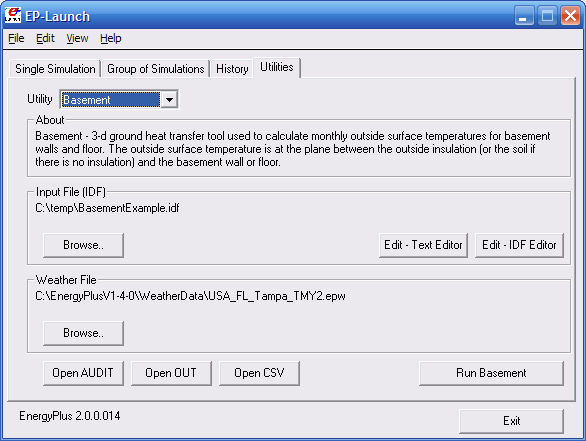
\includegraphics[width=0.9\textwidth, height=0.9\textheight, keepaspectratio=true]{media/image009.png}
\caption{EP-Launch Utilities Tab. \protect \label{fig:ep-launch-utilities-tab.}}
\end{figure}

For each utility, input files can be selected by using the Browse Button. The input file can be opened using a text editor and, for certain utilities, the IDF Editor. If a weather file is needed for a utility it can also be selected. For other utilities, no weather file is needed and that portion of the screen is not shown. The appropriate output files can be opened by the ``Open'' button near the bottom of the screen. To run the utility, use the ``Run'' button in the lower left corner of the screen above the ``Exit'' button.

In addition, for each utility, a brief description of the function of the utility is shown in the about box but much more information is available in the AuxiliaryPrograms documentation.

\subsection{Caveats}\label{caveats}

Remember to save changes made in the editor before you run another simulation.

The simulation cannot write new results to open files which are locked by another application.

You will need to close the spreadsheet program that views the resulting CSV files prior to another simulation and you may need to close the text editor windows also (depending on your editor).

The EPL-RUN.BAT batch file is used to run EnergyPlus from the EP-Launch program. It can be edited with care if other postprocessors or preprocessors are to be used.

\subsection{When things go wrong}\label{when-things-go-wrong}

Though EnergyPlus has had several releases (including beta releases prior to initial release), there still may be problems when input files meet with EnergyPlus. If you are using EP-Launch when this happens, you will see a window appear as in the figure below (Figure~\ref{fig:energyplus-crash-within-ep-launch.}). Follow the instructions listed on the screen.

\begin{figure}[hbtp] % fig 10
\centering
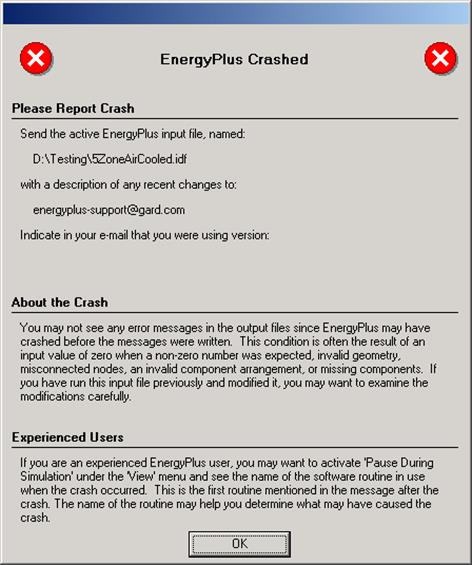
\includegraphics[width=0.9\textwidth, height=0.9\textheight, keepaspectratio=true]{media/image010.jpg}
\caption{EnergyPlus crash within EP-Launch. \protect \label{fig:energyplus-crash-within-ep-launch.}}
\end{figure}

\subsection{Bugs}\label{bugs}

The EP-Launch program has been through several ``releases'' but there is still a chance you will find bugs. Please report them to the energyplus-support@gard.com address so that we can fix them prior to the release.

If the pull-down lists ever are shown as blank the ``reset'' button may be used. This unlabeled button is very small in the lower left-hand corner of the main screen. It removes the items shown in the recently used file list and causes the program to forget the selected viewers and text editors; and exits the program. When you start EP-Launch again, you will need to make these selections (viewers and text editors) again.
